\section{Auswertung der Messdaten}
\label{sec:Auswertung}

\subsection{Kompensation des Erdmagnetfeldes}
Das Erdmagnetfeld wurde mit einem Spulenstrom von $I = \SI{0.231}{\ampere}$
ausgeglichen. Die Parameter der verwendeten Spule sind in Tabelle~\ref{tab:spulendaten}
aufgeführt.
\begin{table}
  \centering
  \caption{Spulenparameter der Helmholtz-Spulen.}
  \label{tab:spulendaten}
  \sisetup{table-format=10.0}
  \begin{tabular}{S S[table-format=3.0] S[table-format=1.5]}
    \toprule
    {Spule} & {Windungszahl $N$} & {Radius $r/\si{\meter}$} \\
    \midrule
    {\text{Sweep}}      &  11 & 0.16390 \\
    {\text{Horizontal}} & 154 & 0.15790 \\
    {\text{Vertikal}}   &  20 & 0.11735 \\
    \bottomrule
  \end{tabular}
\end{table}
Mit der Gleichung~\ref{eqn:helmholtz} kann die magnetische Feldstärke einer
Helmholtzspule berechnet werden. Die vertikale Komponente des
Erdmagnetfeldes ergibt sich demnach zu
\begin{equation}
  B_{v} \approx  \SI{13.9402498}{\micro\tesla}.
  \label{eqn:erdmagnetfeld}
\end{equation}
Der Literaturwert beträgt $B_{v \text{lit}} = \SI{45.355}{\micro\tesla}$~\cite{gfzpotsdam}.

\subsection{Bestimmung der Land\`e-Faktoren}
\label{subsec:lande}
Nach Gleichung~\ref{eqn:helmholtz} lassen sich aus den gemessenen Stromstärken die
Magnetfeldstärken berechnen. Das gesamte
Magnetfeld setzt sich zusammen aus dem Feld der \textit{Sweep}-Spule und dem Feld
der Horizontalspule. Das gesamte Magnetfeld in Abhängigkeit von der RF-Frequenz
ist in Abbildung \ref{fig:magnetfeld1} dargestellt.

\begin{figure}[H]
  \centering
  \includegraphics[scale=0.6]{build/plot1.pdf}
  \caption{Das gesamte Magnetfeld in Abhängigkeit von der Frequenz.}
  \label{fig:magnetfeld1}
\end{figure}
\noindent
In Abbildung \ref{fig:magnetfeld1} wurde eine lineare Regression durchgeführt.
Aus der Steigung dieser kann nach Gleichung \ref{eqn:bf} der gyromagnetische
Faktor bestimmt werden, indem diese zu Gleichung \ref{eqn:gyrom} umgestellt wird.
\begin{equation}
  g_{F} = \frac{h}{m \mu_{B}}.
  \label{eqn:gyrom}
\end{equation}
\noindent
Es ergeben sich die Regressionsparameter
\begin{align}
  m_{87}  & =  \SI{1.422(0.029)e-10}{\tesla\per\hertz}\\
  m_{85}  & =  \SI{2.06(0.12)e-10}{\tesla\per\hertz}.
\end{align}
\noindent
Mit diesen Werten ergeben sich die gyromagnetischen Faktoren
\begin{align}
	g_{87} & = \num{0.502+-0.01}\\
  g_{85} & = \num{0.346+-0.021}.
\end{align}
\noindent

\subsection{Bestimmung des Kernspins der Isotope}
\label{subsec:kernspin}
Unter Verwendung des in Abschnitt \ref{subsec:lande} ermittelten gyromagnetischen
Faktors kann für das jeweilige Isotop der Kernspin ermittelt werden. Da für den
gyromagnetischen Faktor Gleichung \ref{eqn:gyrogyro} gilt, kann durch Einsetzen
der bekannten Werte
\begin{align}
S =\ & \frac{1}{2}, & L =\ & 0, & J =\ & \frac{1}{2}, & F =\ & I + J
\end{align}
der Kernspin ermittelt werden. Es ergeben sich die Kernspins
\begin{align}
	I_{87} = & \num{1.49+-0.04} \\
  I_{85} = & \num{2.39+-0.17}.
\end{align}
Ein Vergleich mit den jeweiligen Literaturwerten \cite{Rb} liefert eine jeweilige Abweichung von
\begin{align}
  \Delta I_{87} =\ & \SI{0.7}{\percent} \\
  \Delta I_{85} =\ & \SI{5}{\percent},
\end{align}
was die bisherige Zuordnung der Peaks zu den jeweiligen Isotopen bestätigt.

\subsection{Bestimmung des Isotopenverhältnisses}
\label{subsec:verhältniss}
Das Verhältnis der beiden Isotope $I_{87}$ und $I_{85}$ kann durch Vermessung
der Peaktiefe der Magnetfeldstärke bestimmt werden. In Abbildung \ref{fig:peakbild}
ist die Transitivität gegen die Magnetfeldstärke aufgetragen. Die RF-Frequenz beträgt $\SI{100}{\kilo\hertz}$.
\begin{figure}
  \centering
  \caption{Ein Oszilloskopbild der Transitivität aufgetragen gegen die Magnetfeldstärke. Der kleinere Peak auf der linken Seite entspricht dem Isotop $^{87}\text{Rb}$, während der größere Peak auf der rechten Seite dem Isotop $^{85}\text{Rb}$ entspricht.}
  \label{fig:peakbild}
  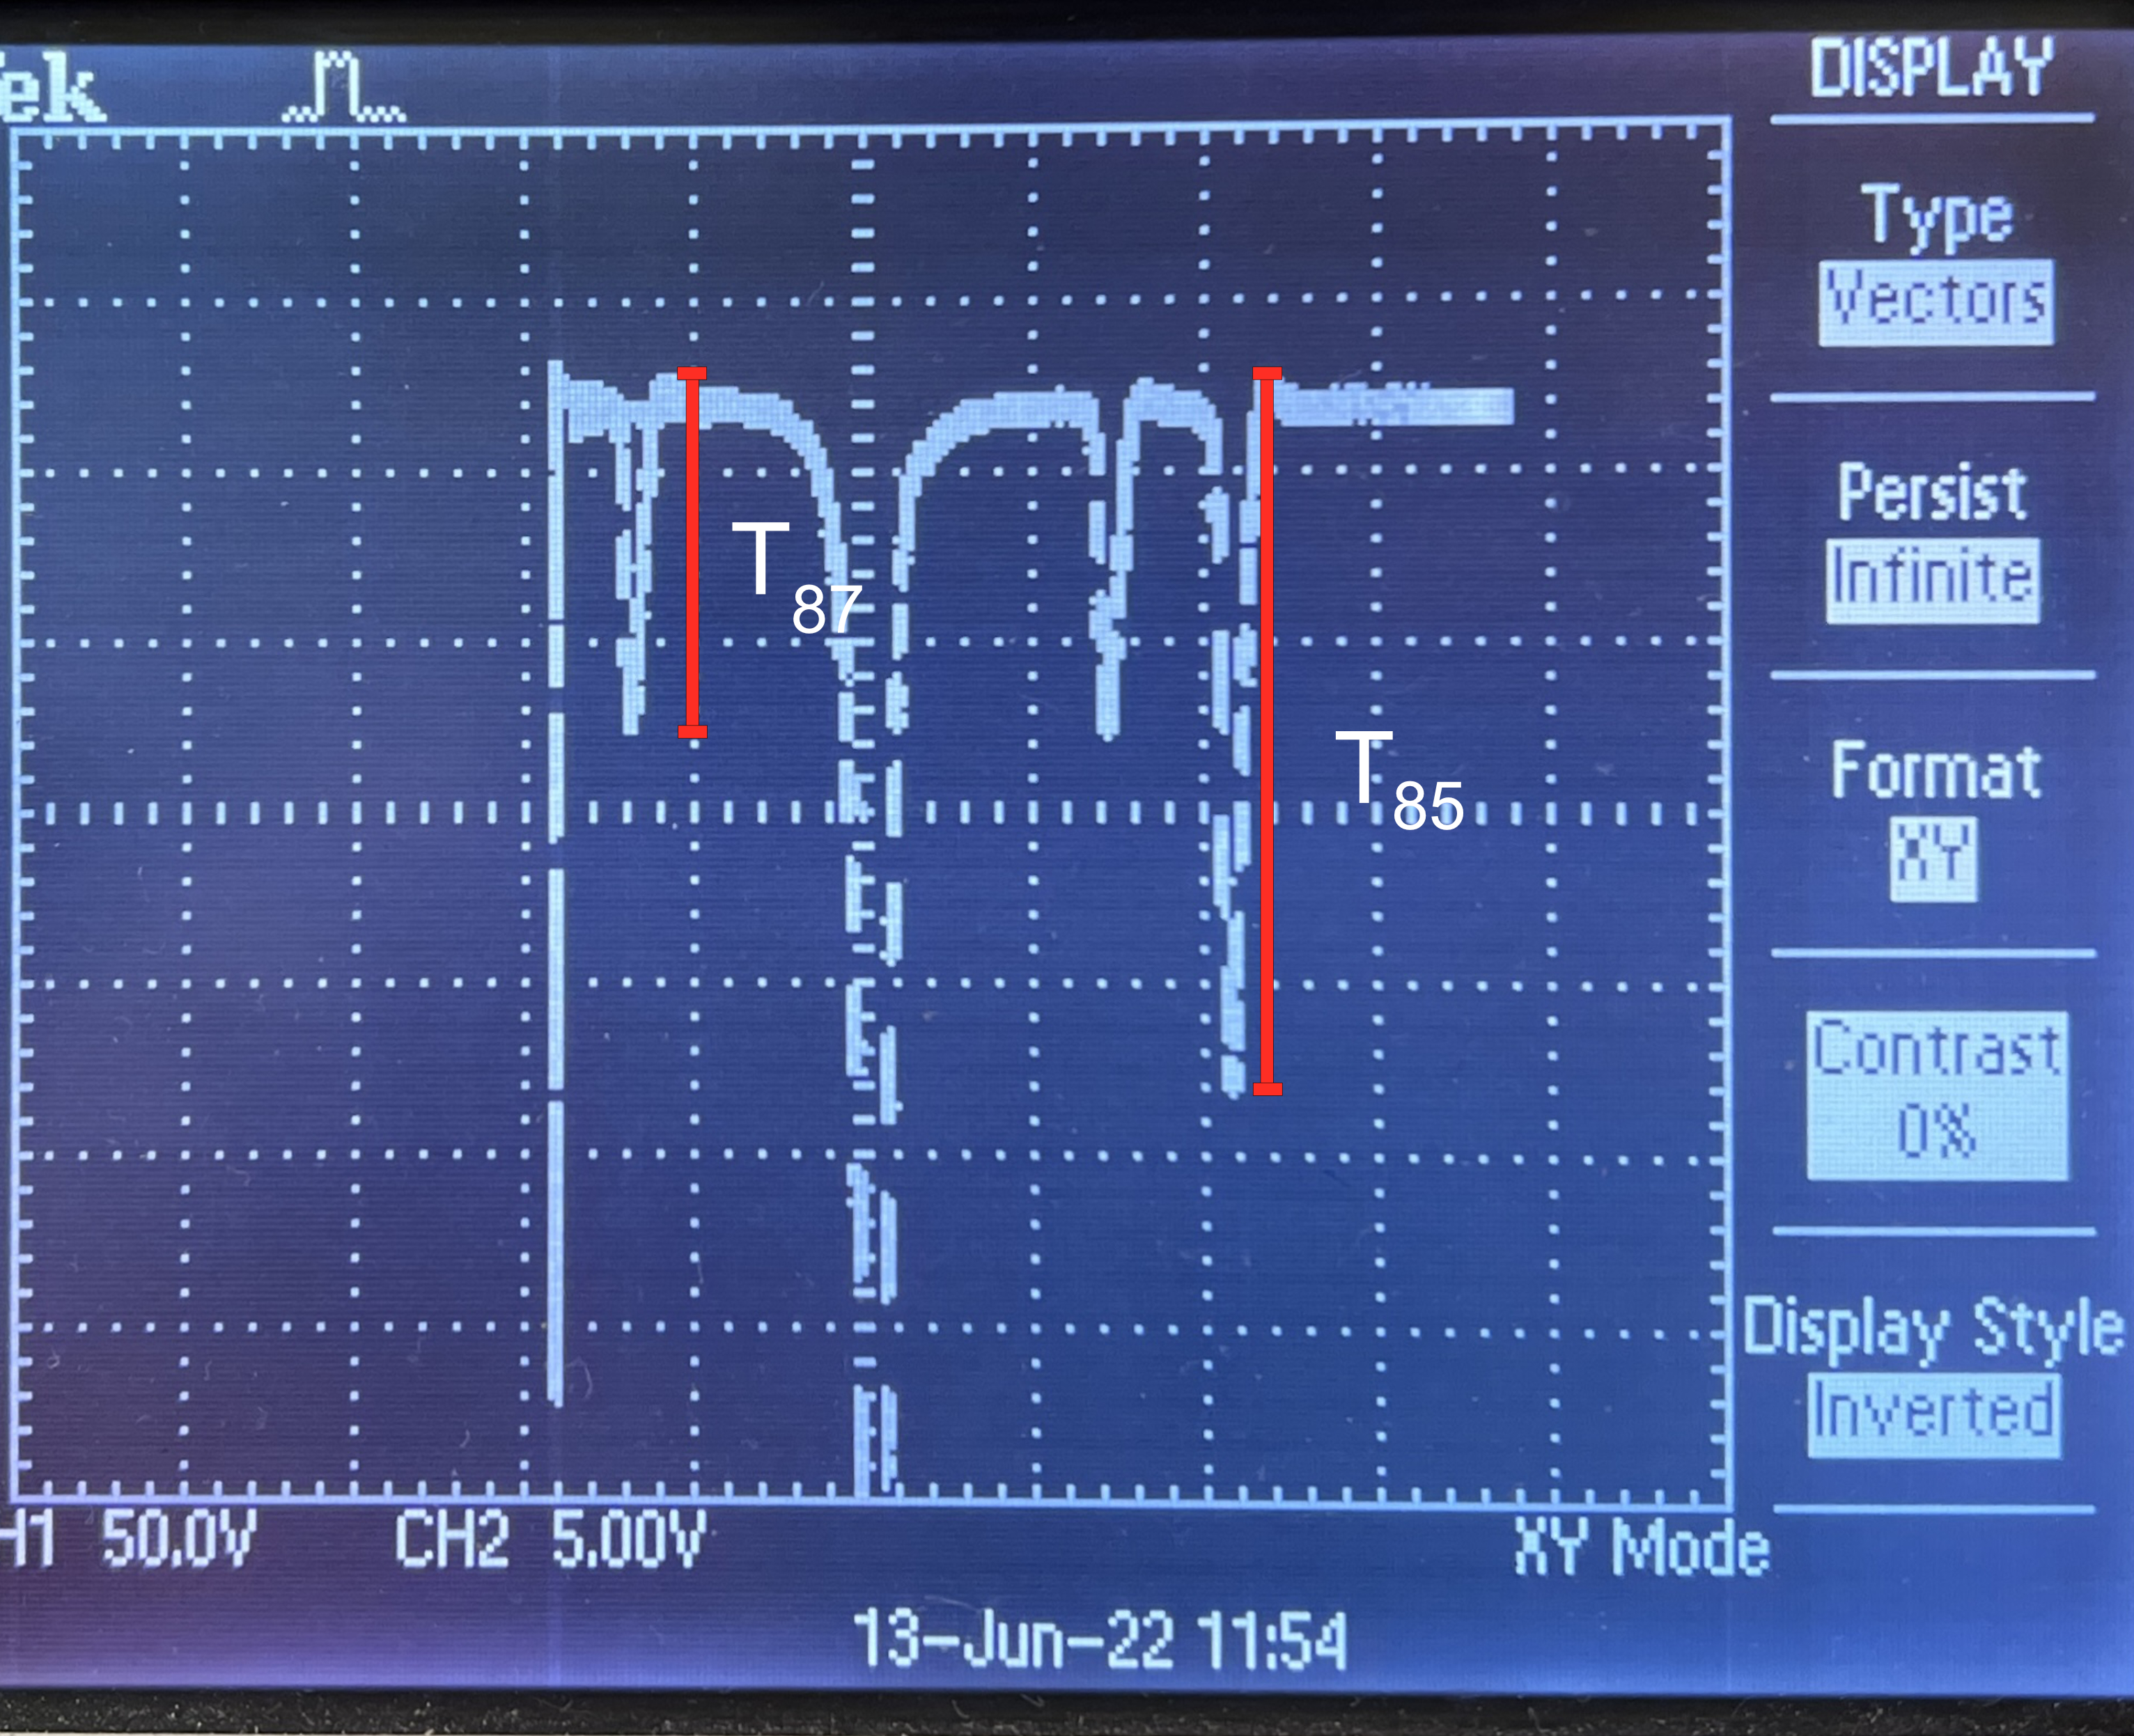
\includegraphics[scale=0.1]{pictures/Peakbild.jpg}
\end{figure}
Eine Vermessung der Peaks wurde mithilfe der Grafik-Software \textit{Affinity Designer} \cite{affinity}
vorgenommen. Es ergeben sich die Peaktiefen
\begin{align}
  T_{87} =\ & \num{524}\, \text{px} \\
  T_{85} =\ & \num{1037}\, \text{px}.
\end{align}
Nach Gleichung \ref{eqn:verhältnis} lassen sich die Isotopenanteile abschätzen:
\begin{equation}
  \label{eqn:verhältnis}
 	A_{i} = \frac{N_{i}}{N_{1} + N_{2}}.
\end{equation}
Es ergeben sich die Anteile
\begin{align}
	A_{87} =\ & \SI{33.56}{\percent} \\
  A_{85} =\ & \SI{66.43}{\percent}.
\end{align}

\subsection{Der Beitrag des quadratischen Zeeman-Effektes}
\label{subsec:zeemanquadrat}
In diesem Versuch wurde bisher angenommen, dass der quadratische Zeeman-Effekt
keinen relevanten Beitrag liefert. Dies soll im Folgenden überprüft werden.
Die Aufspaltung durch den quadratischen Zeeman-Effekt berechnet sich nach Gleichung
\ref{eqn:zeemanquadrat}. Um eine Abschätzung des maximal möglichen Beitrages zu erhalten,
wird das höchste in diesem Versuch erreichte Magnetfeld angenommen.
Daher wird $B = \SI{225}{\micro\tesla}$ verwendet. Die weiteren Werte sind in
Tabelle \ref{tab:wertezeeman} aufgeführt.
\begin{table}[H]
  \centering
  \caption{Verwendete Werte zur Berechnung des Beitrages des quadratischen Zeeman-Effektes.}
  \label{tab:wertezeeman}
  \sisetup{table-format=3.1}
  \begin{tabular}{S S S}
    \toprule
    {Größe} & {$^{87} Rb$} & {$^{85} Rb$} \\
    \midrule
    $g_{F}$ & $\num{0.502+-0.010}$ & $\num{0.346+-0.021}$ \\
    $M_{F}$ & 2 & 3 \\
   % $\Delta E_{\text{Hyperfein}}$ & \SI{4.53e-24}{\joule} & \SI{2.01e-24}{\joule} \\
    \bottomrule
  \end{tabular}
\end{table}
\noindent
Für die Aufspaltungen in die Hyperfeinstruktur wurden die Werte $\Delta E_{\text{Hyperfein}}= \SI{4.53e-24}{\joule}$
für $ ^{87}Rb $ sowie $\Delta E_{\text{Hyperfein}}= \SI{2.01e-24}{\joule}$ für $^{85}Rb$ verwendet \cite{V21}.
Es ergeben sich für den quadratischen Zeeman-Effekt die Aufspaltungen
\begin{align}
	\Delta E_{Z, ^{87}Rb} =\ & \SI{-2.73+-0.11e-30}{\joule}\\
	\Delta E_{Z, ^{85}Rb} =\ & \SI{-5.8+-0.7e-31}{\joule}.
\end{align}
Zum Vergleich wurden auch die Aufspaltungen aufgrund des linearen Zeeman-Effektes bestimmt:
\begin{align}
	\Delta E_{Z, ^{87}Rb, \text{linear}} =\ & \SI{1.049+-0.021e-27}{\joule}\\
	\Delta E_{Z, ^{85}Rb, \text{linear}} =\ & \SI{7.2+-0.4e-28}{\joule}.
\end{align}
Die linearen Terme liegen also mehrere Größenordnungen über den Beiträgen des
quadratischen Zeeman-Effektes.
